
\documentclass{beamer}
\usepackage{graphicx}
\usepackage{amsmath}
\usetheme{metropolis}
\usepackage{multirow}
\usepackage{tabularx}
\usepackage{amsthm}

\hypersetup{
	colorlinks=true,
	linkcolor=blue,
	filecolor=blue,      
	urlcolor=blue,
	citecolor=blue,
}
\usepackage{natbib}
\bibliographystyle{chicago}

\theoremstyle{plain}
\newtheorem{thm}{Theorem}[section]
\newtheorem{lem}[thm]{Lemma}
\newtheorem{prop}{Proposition}
\newtheorem*{cor}{Corollary}
\newtheorem{assumption}{Assumption}


\title{The Missing Middle in Superstars: Research Proposal}
\author{James Macek}
\begin{document}

\begin{frame}[plain]
	\maketitle
\end{frame}

\begin{frame}{Motivation}
\includegraphics[width = \textwidth]{MMH_Diagram_Landing_Page-2.jpg}
\end{frame}

\begin{frame}{Motivation: Los Angeles}
\includegraphics[width = \textwidth]{LAskyview.png}
\copyright Not Just Bikes
\end{frame}

\begin{frame}{(Eventual) Research Questions}
\begin{enumerate}
	\itemsep1em
 	\item What are the welfare consequences of filling in this missing middle, either by subsidizing construction or rezoning single family neighbourhoods? \pause
 	\item How do they differ across income groups? \pause
 	\item Why target the missing middle and not other types of housing, such as large apartment buildings \citep{asquithetallocaleffects}?
\end{enumerate}
\begin{itemize}
	\item Structural GE model $\implies$ convincing welfare estimates where household mobility plays first order role
	\item Tiebout sorting or congestion/agglomeration externalities.
\end{itemize}
\end{frame}

\begin{frame}{In this talk...} 
\begin{itemize}
	\itemsep1em
	\item Purpose: to fix ideas and provide some motivation for further study. \pause 
	\item Provides a series of empirical observations that show:
	\begin{enumerate}
		\itemsep1em
		\color{black}
		\item Superstar cities differ the most in very high and very low density structures, but not as much in medium density ones. \pause
		\item Appears to be related to the within-city distribution of housing unit density. \pause
		\item It accompanies stronger residential sorting on income. 
	\end{enumerate}
\end{itemize}
\end{frame}

\begin{frame}{In this talk...}
	\begin{itemize}
		\itemsep1em
		\item Provides a simple theory that stitches some of these observations together and discusses consequences for welfare inequality: \pause
		\begin{enumerate}
			\itemsep1em
			\color{black}
			\item  Minimum lot sizes induce a minimum quality of housing. This minimum quality is endogenously higher in superstars.  \pause
			\item Implies \color{blue}low \color{black} density neighborhoods are relatively \color{blue} less \color{black} dense in superstars. \color{red}High \color{black} density neighborhoods are relatively \color{red}more  \color{black} dense. This is in line with empirical evidence.\pause
			\item Creates additional consumption inequality. Households with income below an endogenous cut-off are made relatively worse off than those above. This cut-off is generally higher in superstars.
		\end{enumerate}
	\end{itemize}
\end{frame}

\begin{frame}{Literature}
\fontsize{8pt}{7.2}	
\begin{itemize}
	\itemsep4em
\item \color{red} Residential income sorting, segregation and/or inequality in cities \color{black} \cite{Coutureetal}, \cite{parispoor},  \cite{urbanrevival}, \cite{su2021}, \cite{endogentrification}, \cite{FogliGuerrieri}, \cite{ineqcitysize}, \cite{spatialsorting}, \cite{bshartley2020}

\item \color{purple} Zoning + Housing Supply + Regulation + Affordability \color{black} \cite{keepingpeopleout}, \cite{calabresetal}, \cite{Hamilton1975}, \cite{hamilton1976}, \cite{gyourkomolloy}, \cite{superstarcities}, \cite{mastwarding}, \cite{turner2014}, \cite{bbheight}, \cite{spatialSizeofUSUrbAreas}, \cite{gyourkovoith1997}, \cite{BSH}, \cite{hilber2021} \cite{HILBER2013}, \cite{op2014}, \cite{davidoff2022}, \cite{saiz2010}, \cite{griesonwhite}, Kulka (2019), Song (2021), Parkhomenko (2020), \cite{mastspillovers}, \cite{asquithetallocaleffects}, \cite{albouyetal}


\item \color{teal} Quantitative spatial models \color{black} \cite{quantspatial}, \cite{berlinwall}, \cite{transportinfrastructure}, Allen, Arkolakis and Li (2016), Acosta (2021), Herzog (2022). 
\end{itemize}
\end{frame}

\begin{frame}{Fact 1: Disproportionate differences in high density structures}
 \includegraphics[width = \textwidth]{structure_type_dist.png}
\end{frame}

\begin{frame}{Fact 2: Stronger income sorting on structure density}
\includegraphics[width = \textwidth]{structure_type_income.png}
\end{frame}

\begin{frame}{Fact 3: Implications for the housing unit density distribution}
\begin{itemize}
	\color{black}
	\item Idea: if
	\begin{enumerate}
		\item There is spatial correlation in the locations of high density structures (i.e. large condominiums concentrated downtown) \pause
		\item and high density structures are disproportionately represented in superstars
	\end{enumerate}
\item Then, high density locations\footnote{Here, I'm measuring density as the number of housing units per unit of land.} might be relatively higher density in superstars. 
\item Same logic could be applied to \color{red} medium \color{black} density structures, so that \textit{\color{red} medium \color{black} density locations are relatively less dense in superstars.}
\item This is what I find!
\end{itemize}
\end{frame}

\begin{frame}{Fact 3: Implications for the housing unit density distribution}
\begin{itemize}
	\color{black}
	\item Using tract level data from the 2010 Census \pause
	\item Within each MSA, I rank tracts by their density of housing units. Ranking lies in the unit interval. \pause
	\item I flexibly regress tract-level housing unit density against this ranking separately for both the superstar and non-superstar samples. \pause
	\item Housing unit density is \color{red} normalized to be on average 1 \color{black} across tracts within each MSA. Controls for MSA fixed effects. 
\end{itemize}
\end{frame}

\begin{frame}{Fact 3: Implications for the housing unit density distribution}
	\begin{figure}
		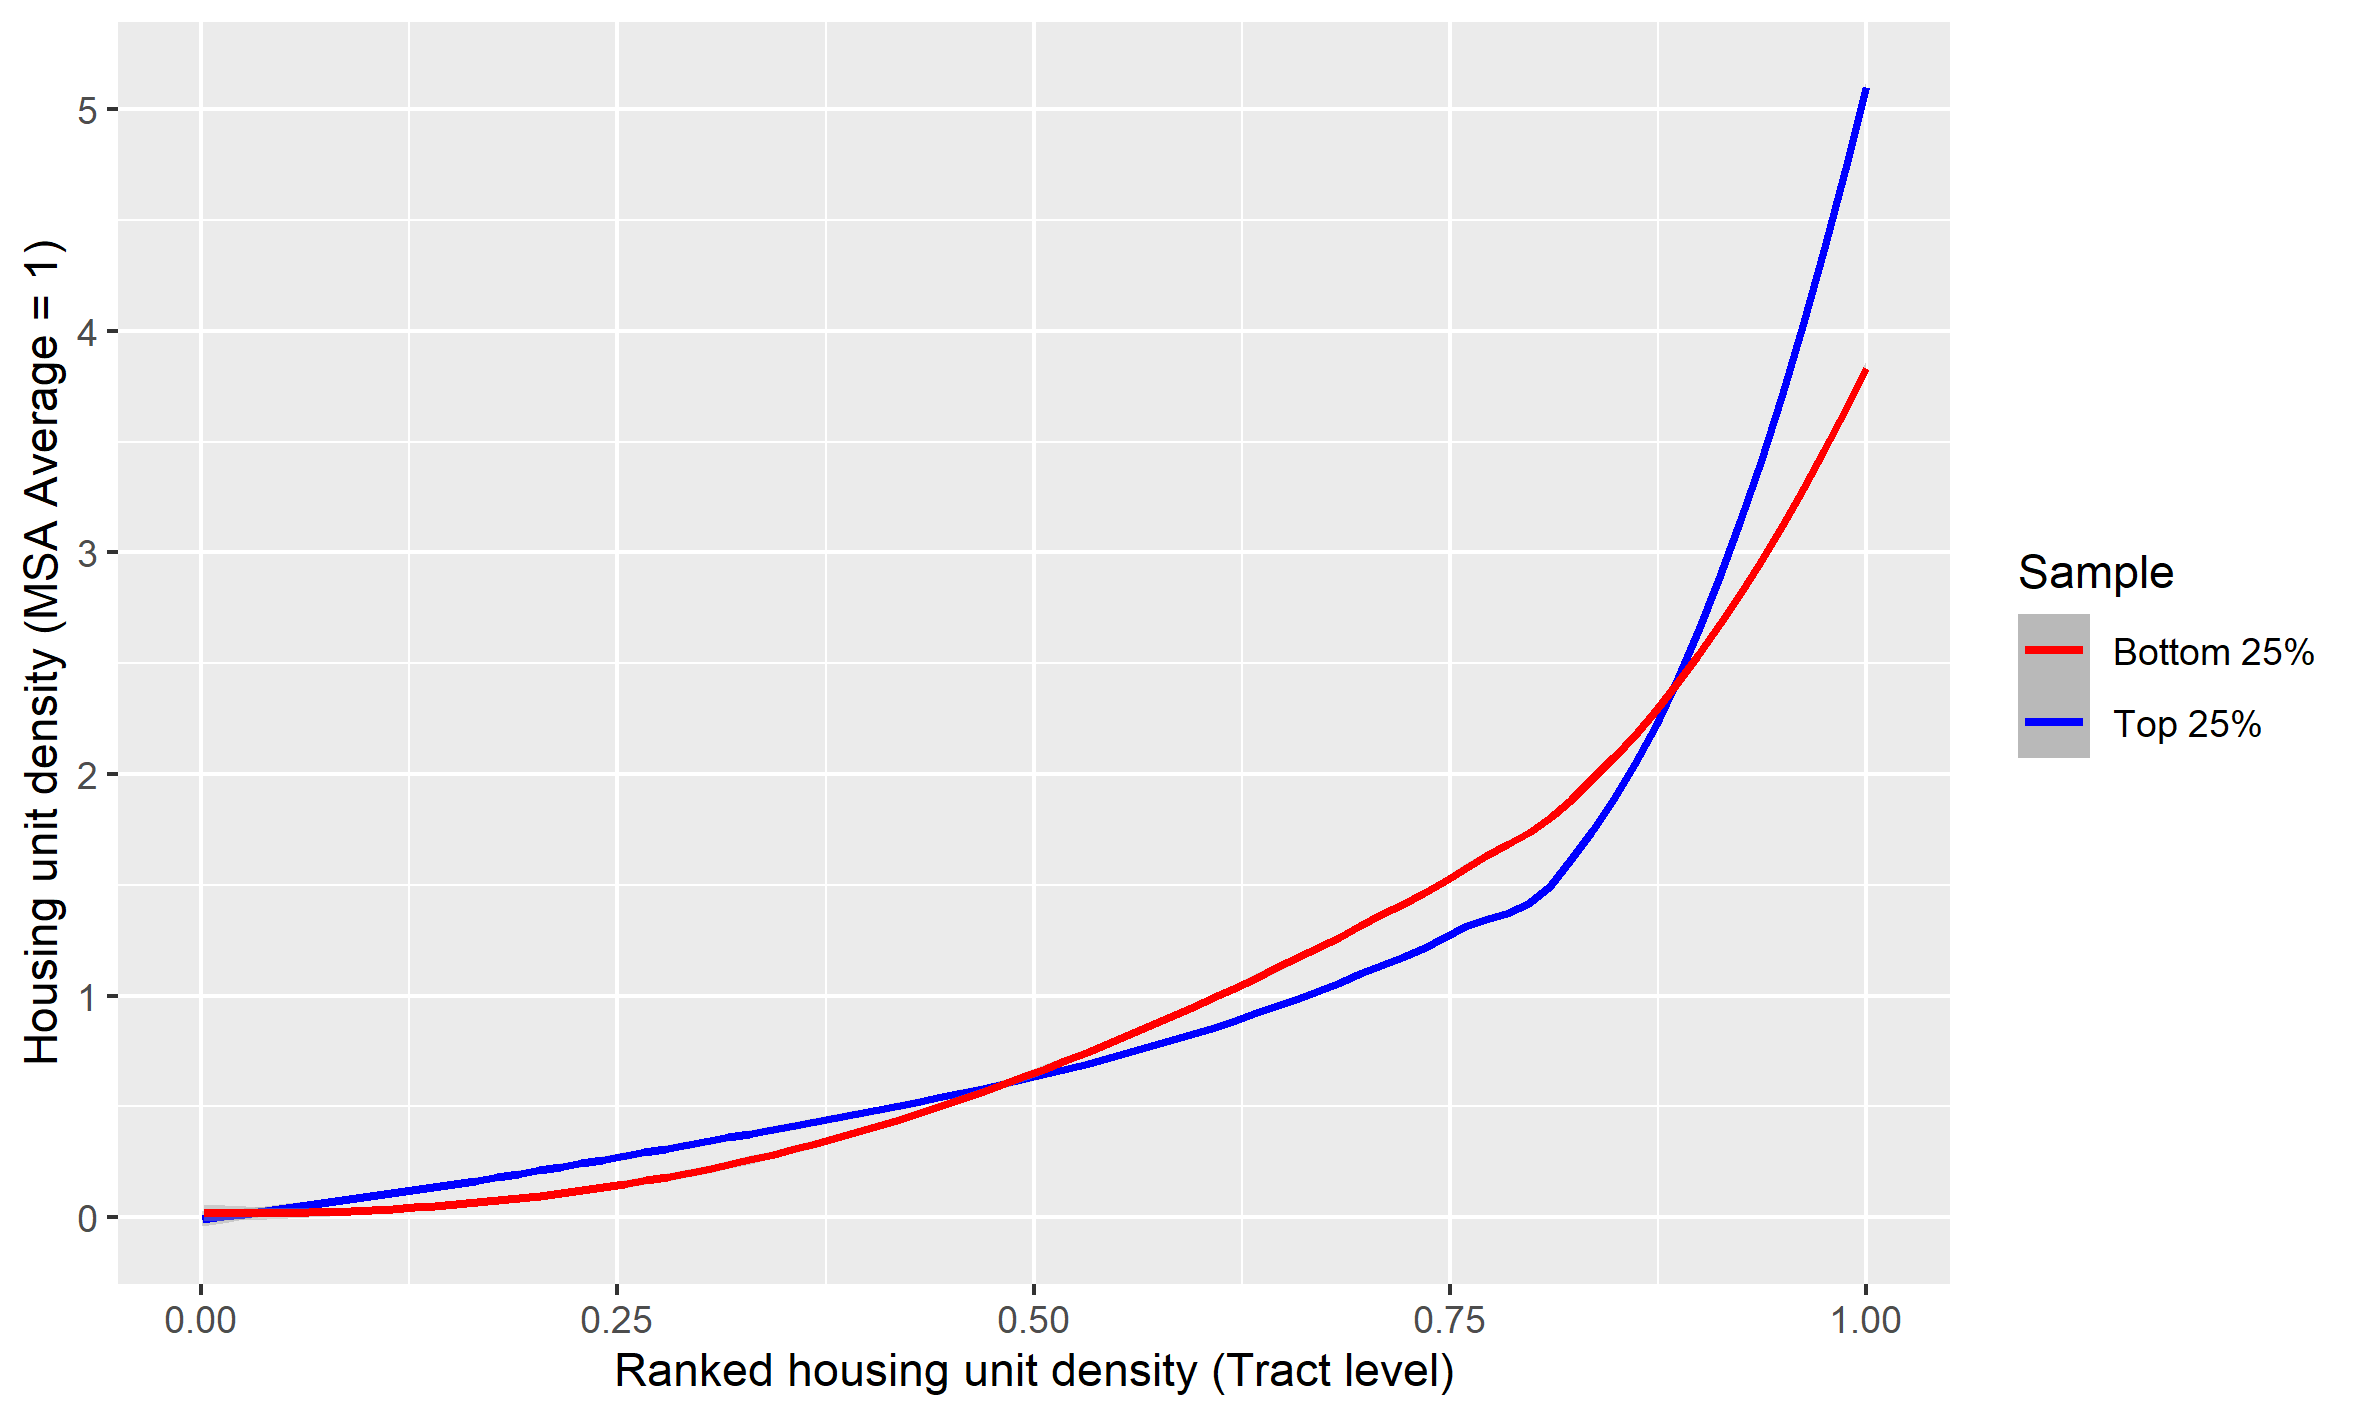
\includegraphics[width=\textwidth]{tractdens_dist.png}
	\end{figure}

\end{frame}


\begin{frame}{Fact 3:}
\begin{itemize}
	\color{black}
	\item The shape of the distribution \textit{may not} be driven the presence of different types of structures, suggesting the missing middle is irrelevant. 
	\item To delve deeper, I linearly decompose housing unit density $D_{H, im}$ into three margins:
	\begin{equation}
		D_{H, im} = D_{S, im} + D_{M, im} + D_{L, im}
	\end{equation}
\item where $D_{S, im}$ is the number of single family homes in MSA $m$ and tract $i$ divided by the total land mass of the tract. 
\item $D_{M, im}$ and $D_{L, im}$ are defined analogously for structures with 2-19 housing units and 20+ units, respectively. Call them Middle and High density components. 
\item \color{red} Repeat \color{black} the regression for each component separately. Justified because the conditional expectation is additive.
\end{itemize}	
\end{frame}

\begin{frame}{Fact 3:}
	\centerline{	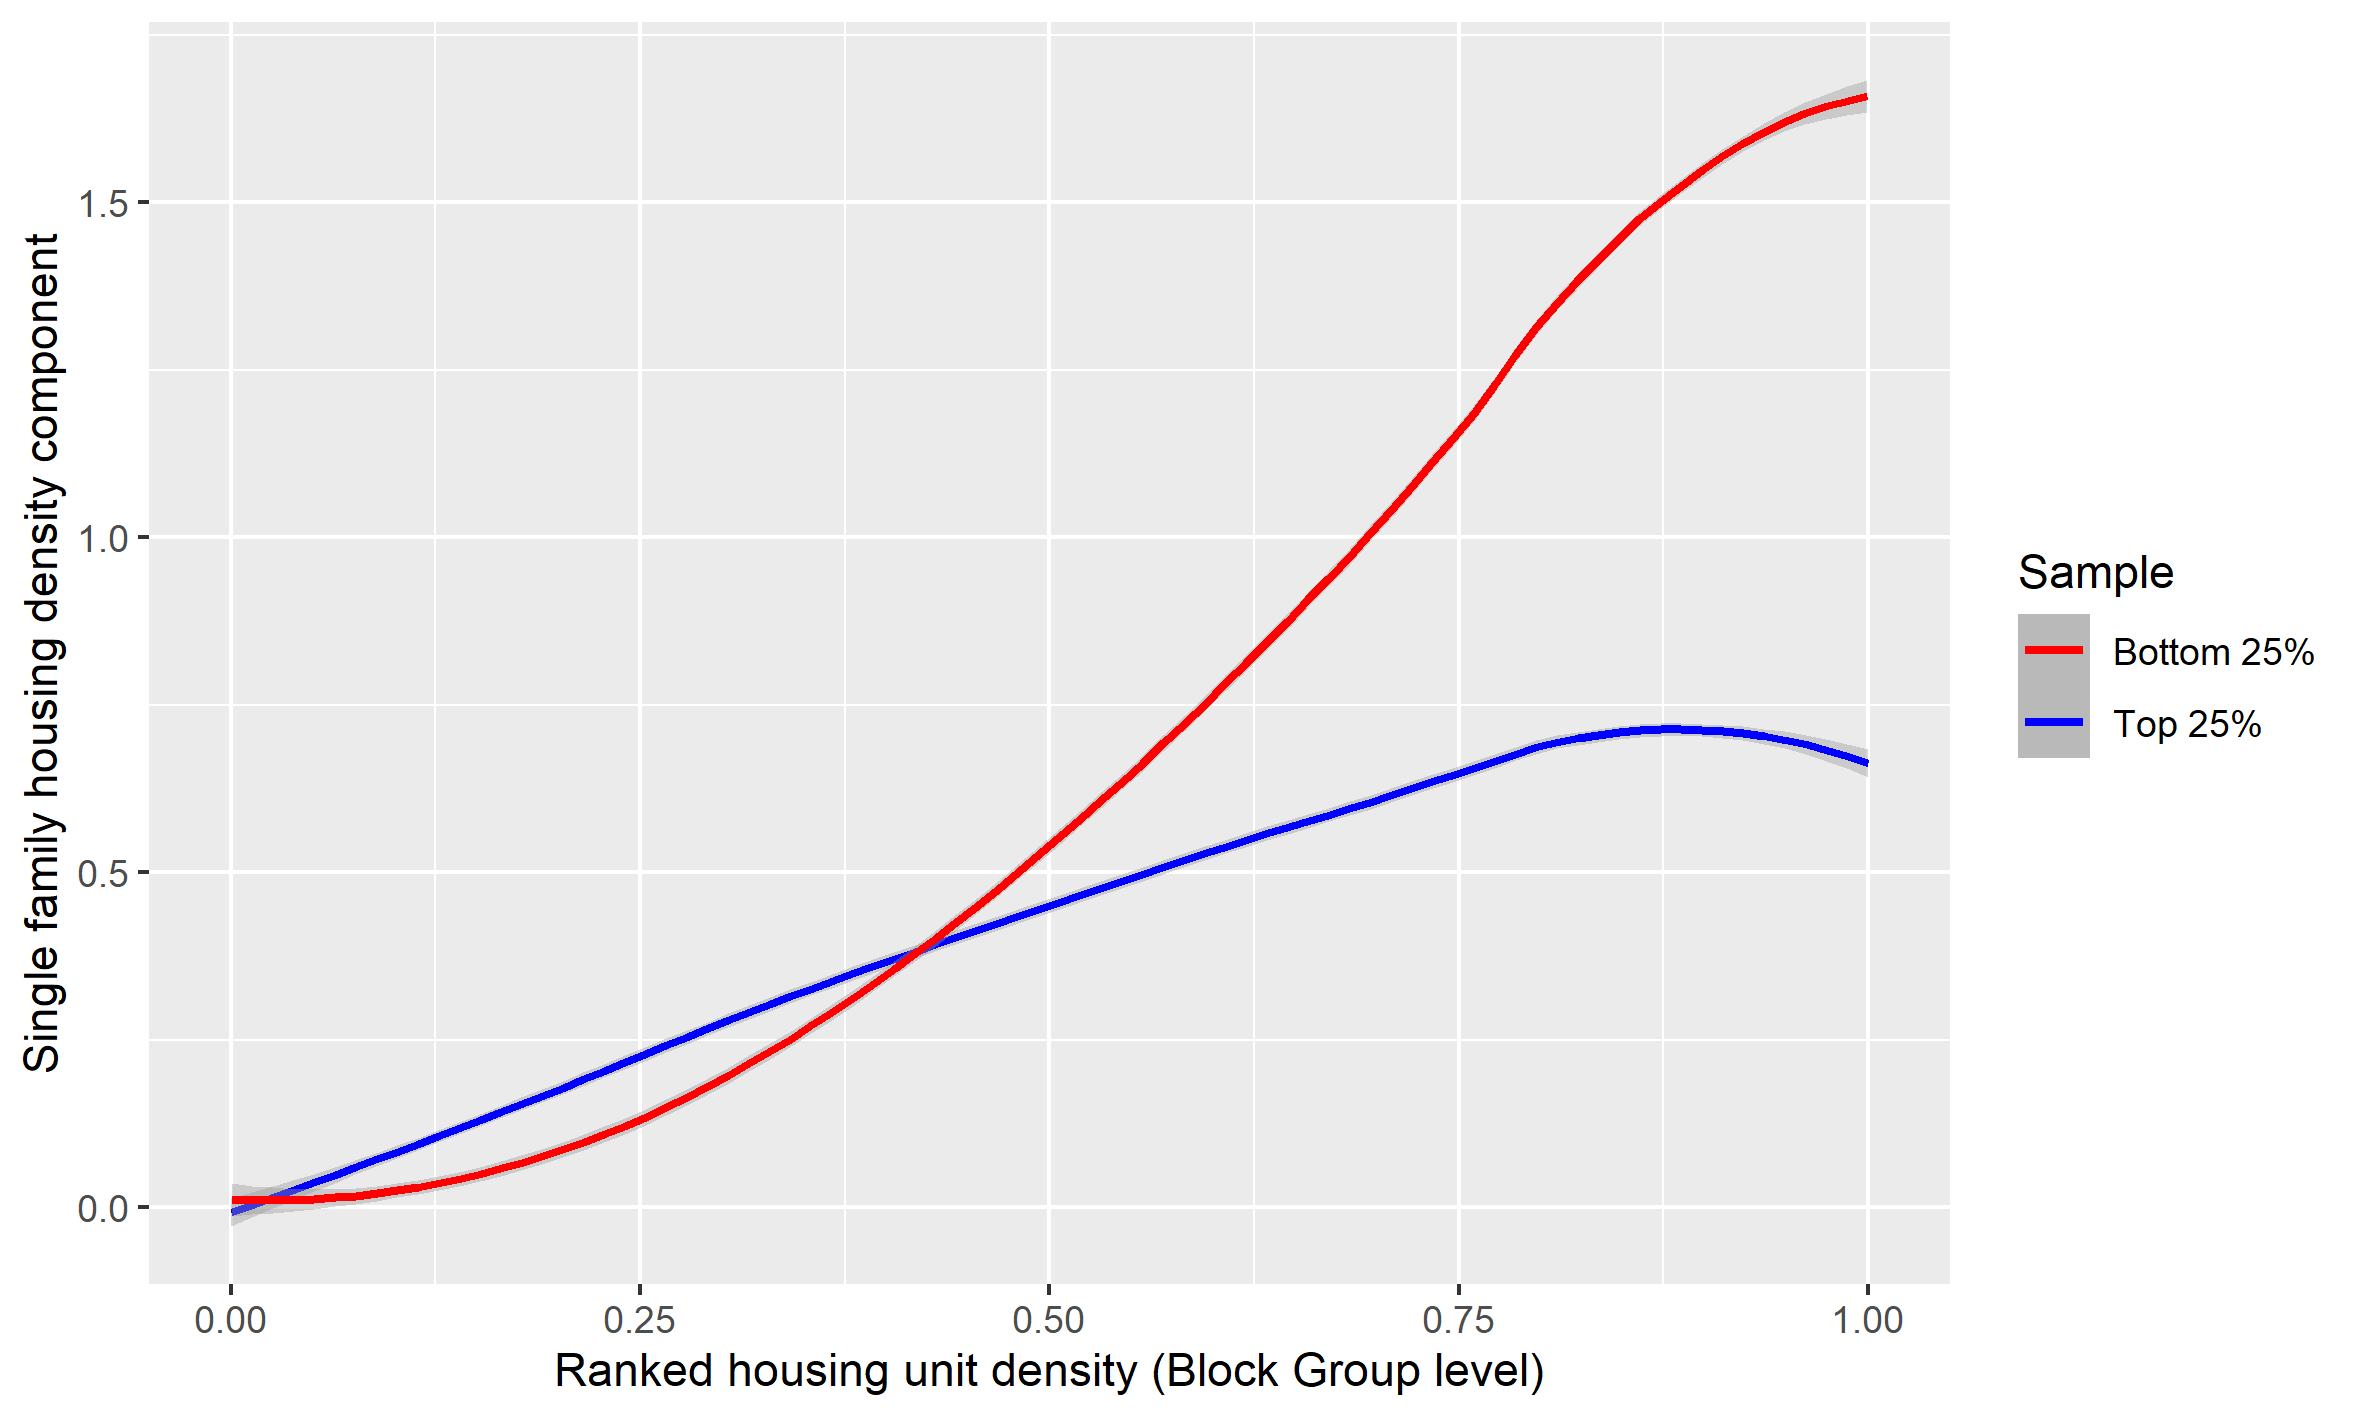
\includegraphics[width=0.7\textwidth, height=0.33\textheight]{singlefamily_dist.png}}
\centerline{	
	\includegraphics[width=0.7\textwidth, height=0.33\textheight]{219building_dist.png}}
\centerline{	
	\includegraphics[width=0.7\textwidth, height=0.33\textheight]{20building_dist.png}}
\end{frame}

\begin{frame}{Fact 3:}
\begin{itemize}
	\color{black}
	\item Takeaways: 
	\begin{enumerate}
		\itemsep1em
		\item Above the 50th percentile, the single family margin is pushing down housing unit density in superstars. The middle and high density margins are not large enough to compensate below the 90th percentile.
		\item Perhaps surprisingly, the medium density components look very similar across samples. 
		\item Could point toward low density single family housing crowding out other types of housing in this region (The Missing Middle!)
	\end{enumerate}
\end{itemize}	
\end{frame}

\begin{frame}{Fact 3:}
\begin{itemize}
	\color{black}
	\item This may not be enough. \textit{Why} is the single family component driving down density in these tracts? Two reasons:
	\begin{enumerate}
		\itemsep1em
		\item  Single family homes occupy a lot of land, but they are low density (Missing Middle)
		\item Single family homes are high density, but they occupy a small fraction of tract land (Not Missing Middle)
	\end{enumerate}
\end{itemize}	
\end{frame}

\begin{frame}{Fact 3:}
\begin{itemize}
\color{black}
\item Log-linearly decompose the single family component into \textit{density} and \textit{land} margins, respectively: 
\begin{equation}
	log(D_{S, im}) = log(\tilde{D}_{S, im}) + log(L_{S, im})
\end{equation}
\item where $\tilde{D}_{S, im}$ is the number of single family homes divided by the total land used for single family housing, and $L_{S, im}$ is the fraction of tract land used for single family housing. 
\item \color{red} Repeat the regression for each component separately. \color{black}
\item National Land Cover Database (NLCD) satellite data. Use "light" and "medium" development as empirical proxy to $L_{S, im}$. 
\end{itemize}
\end{frame}

\begin{frame}{Fact 3:}
	\centerline{	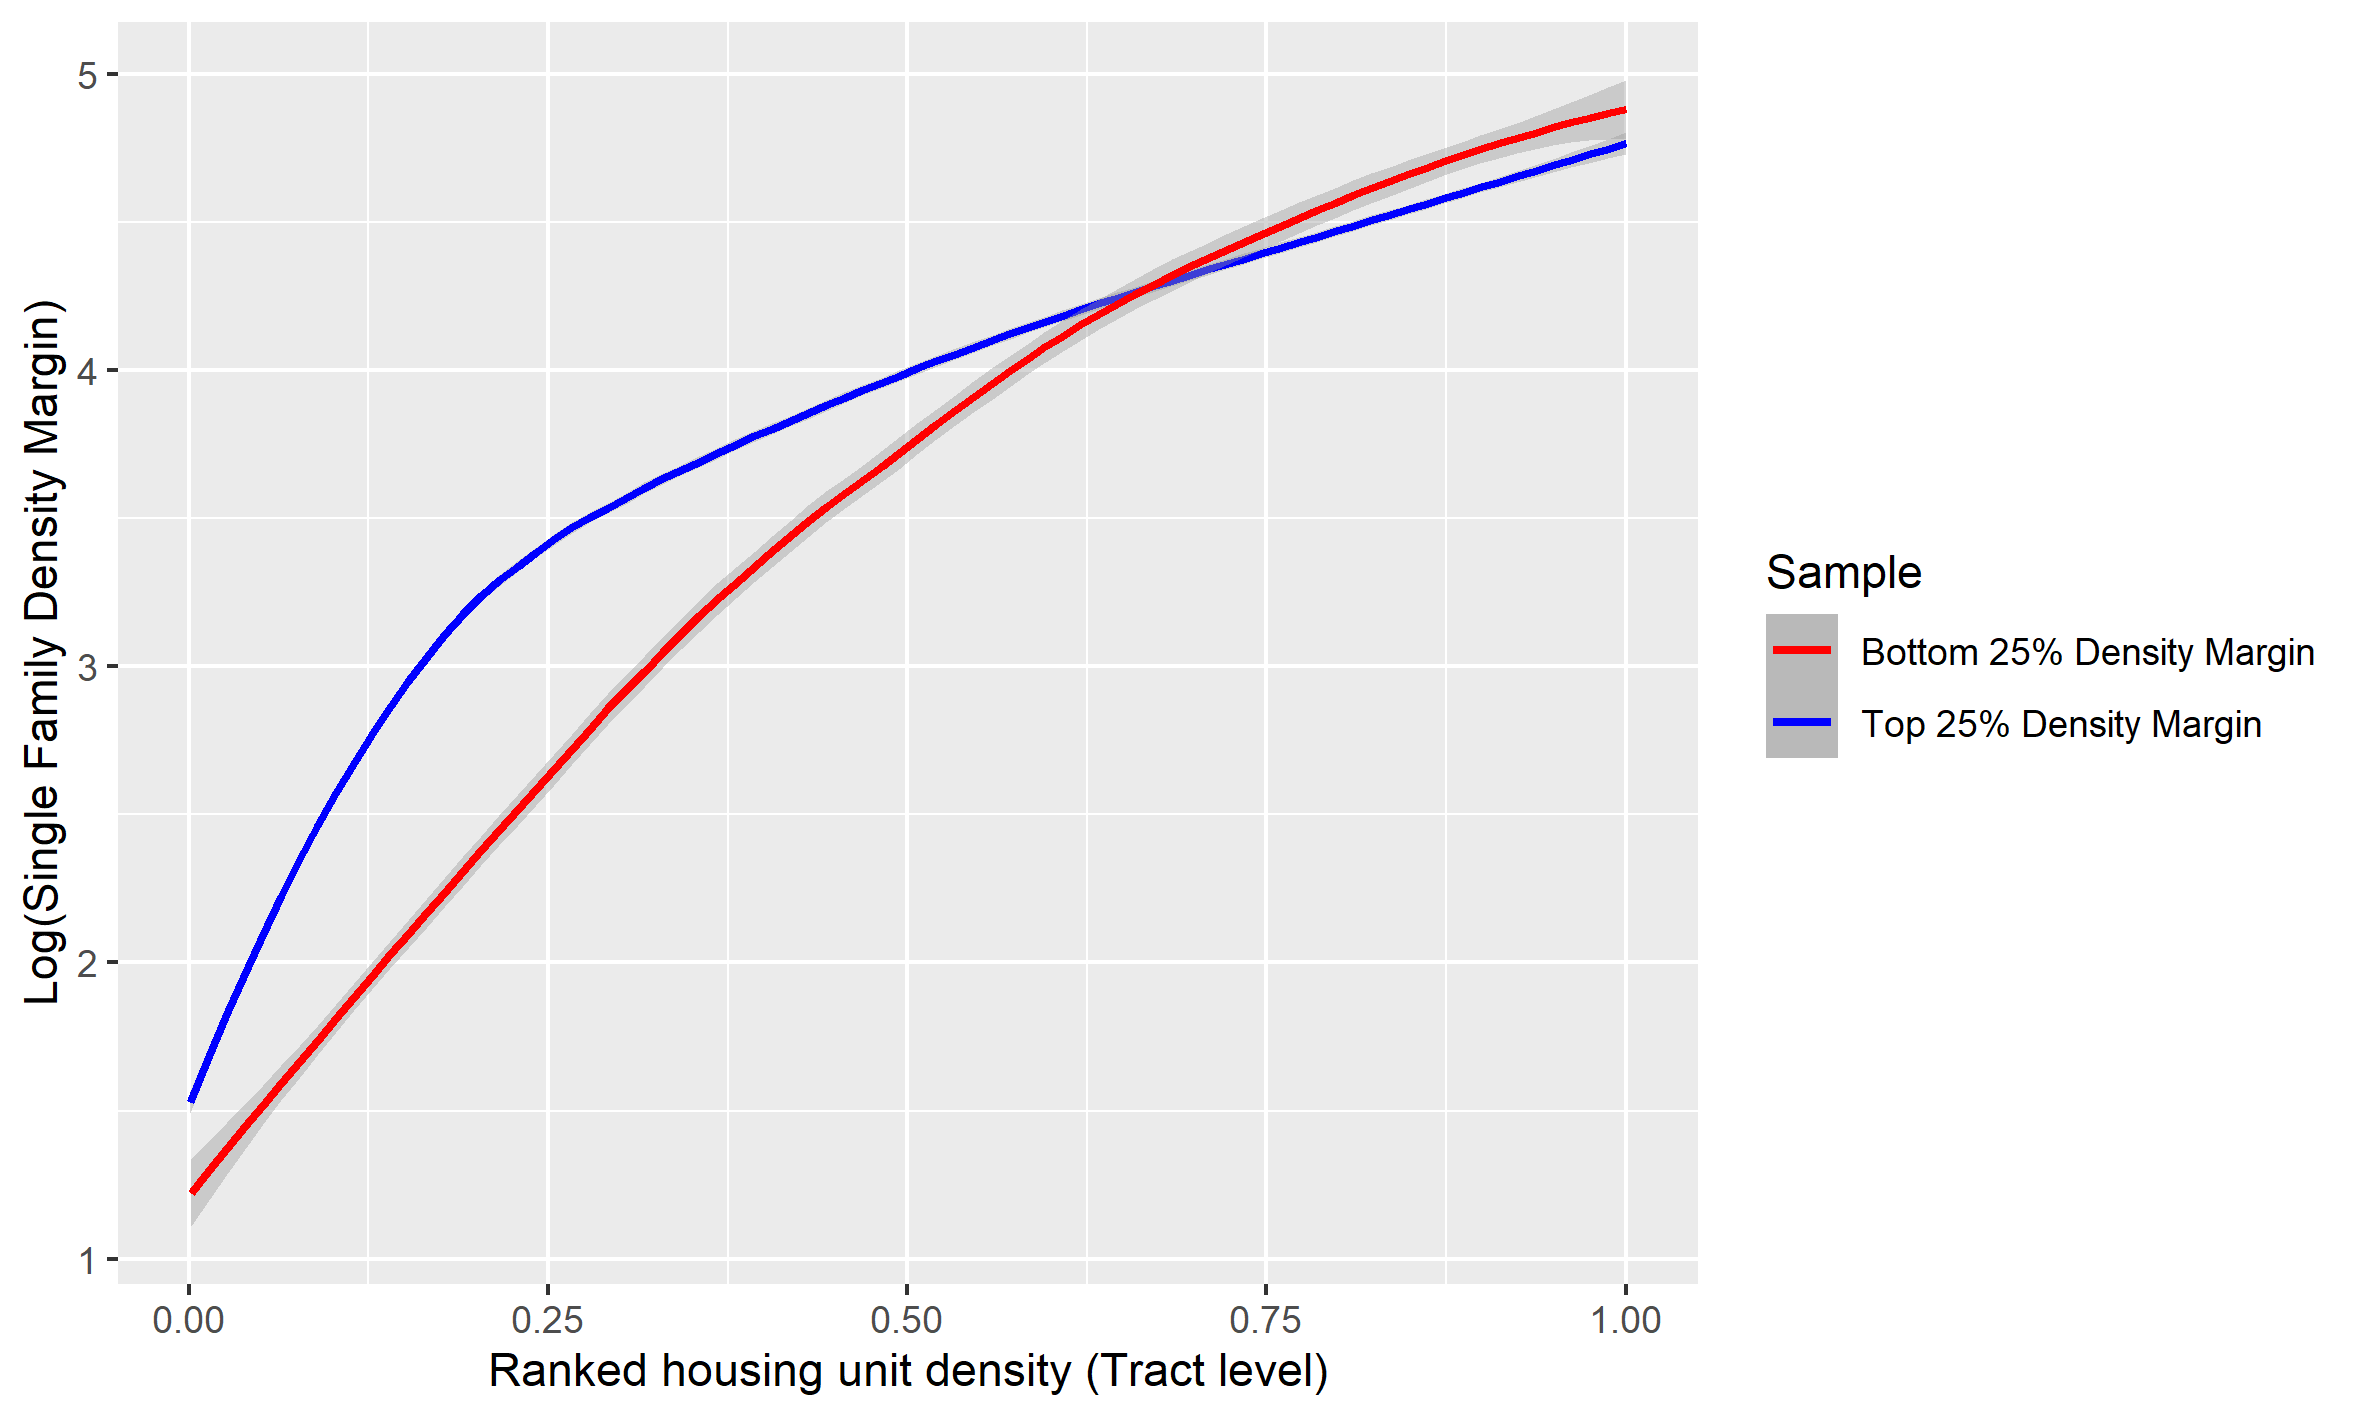
\includegraphics[width=0.7\textwidth, height=0.5\textheight]{SingleFamilyDensity.png}}
\centerline{	
	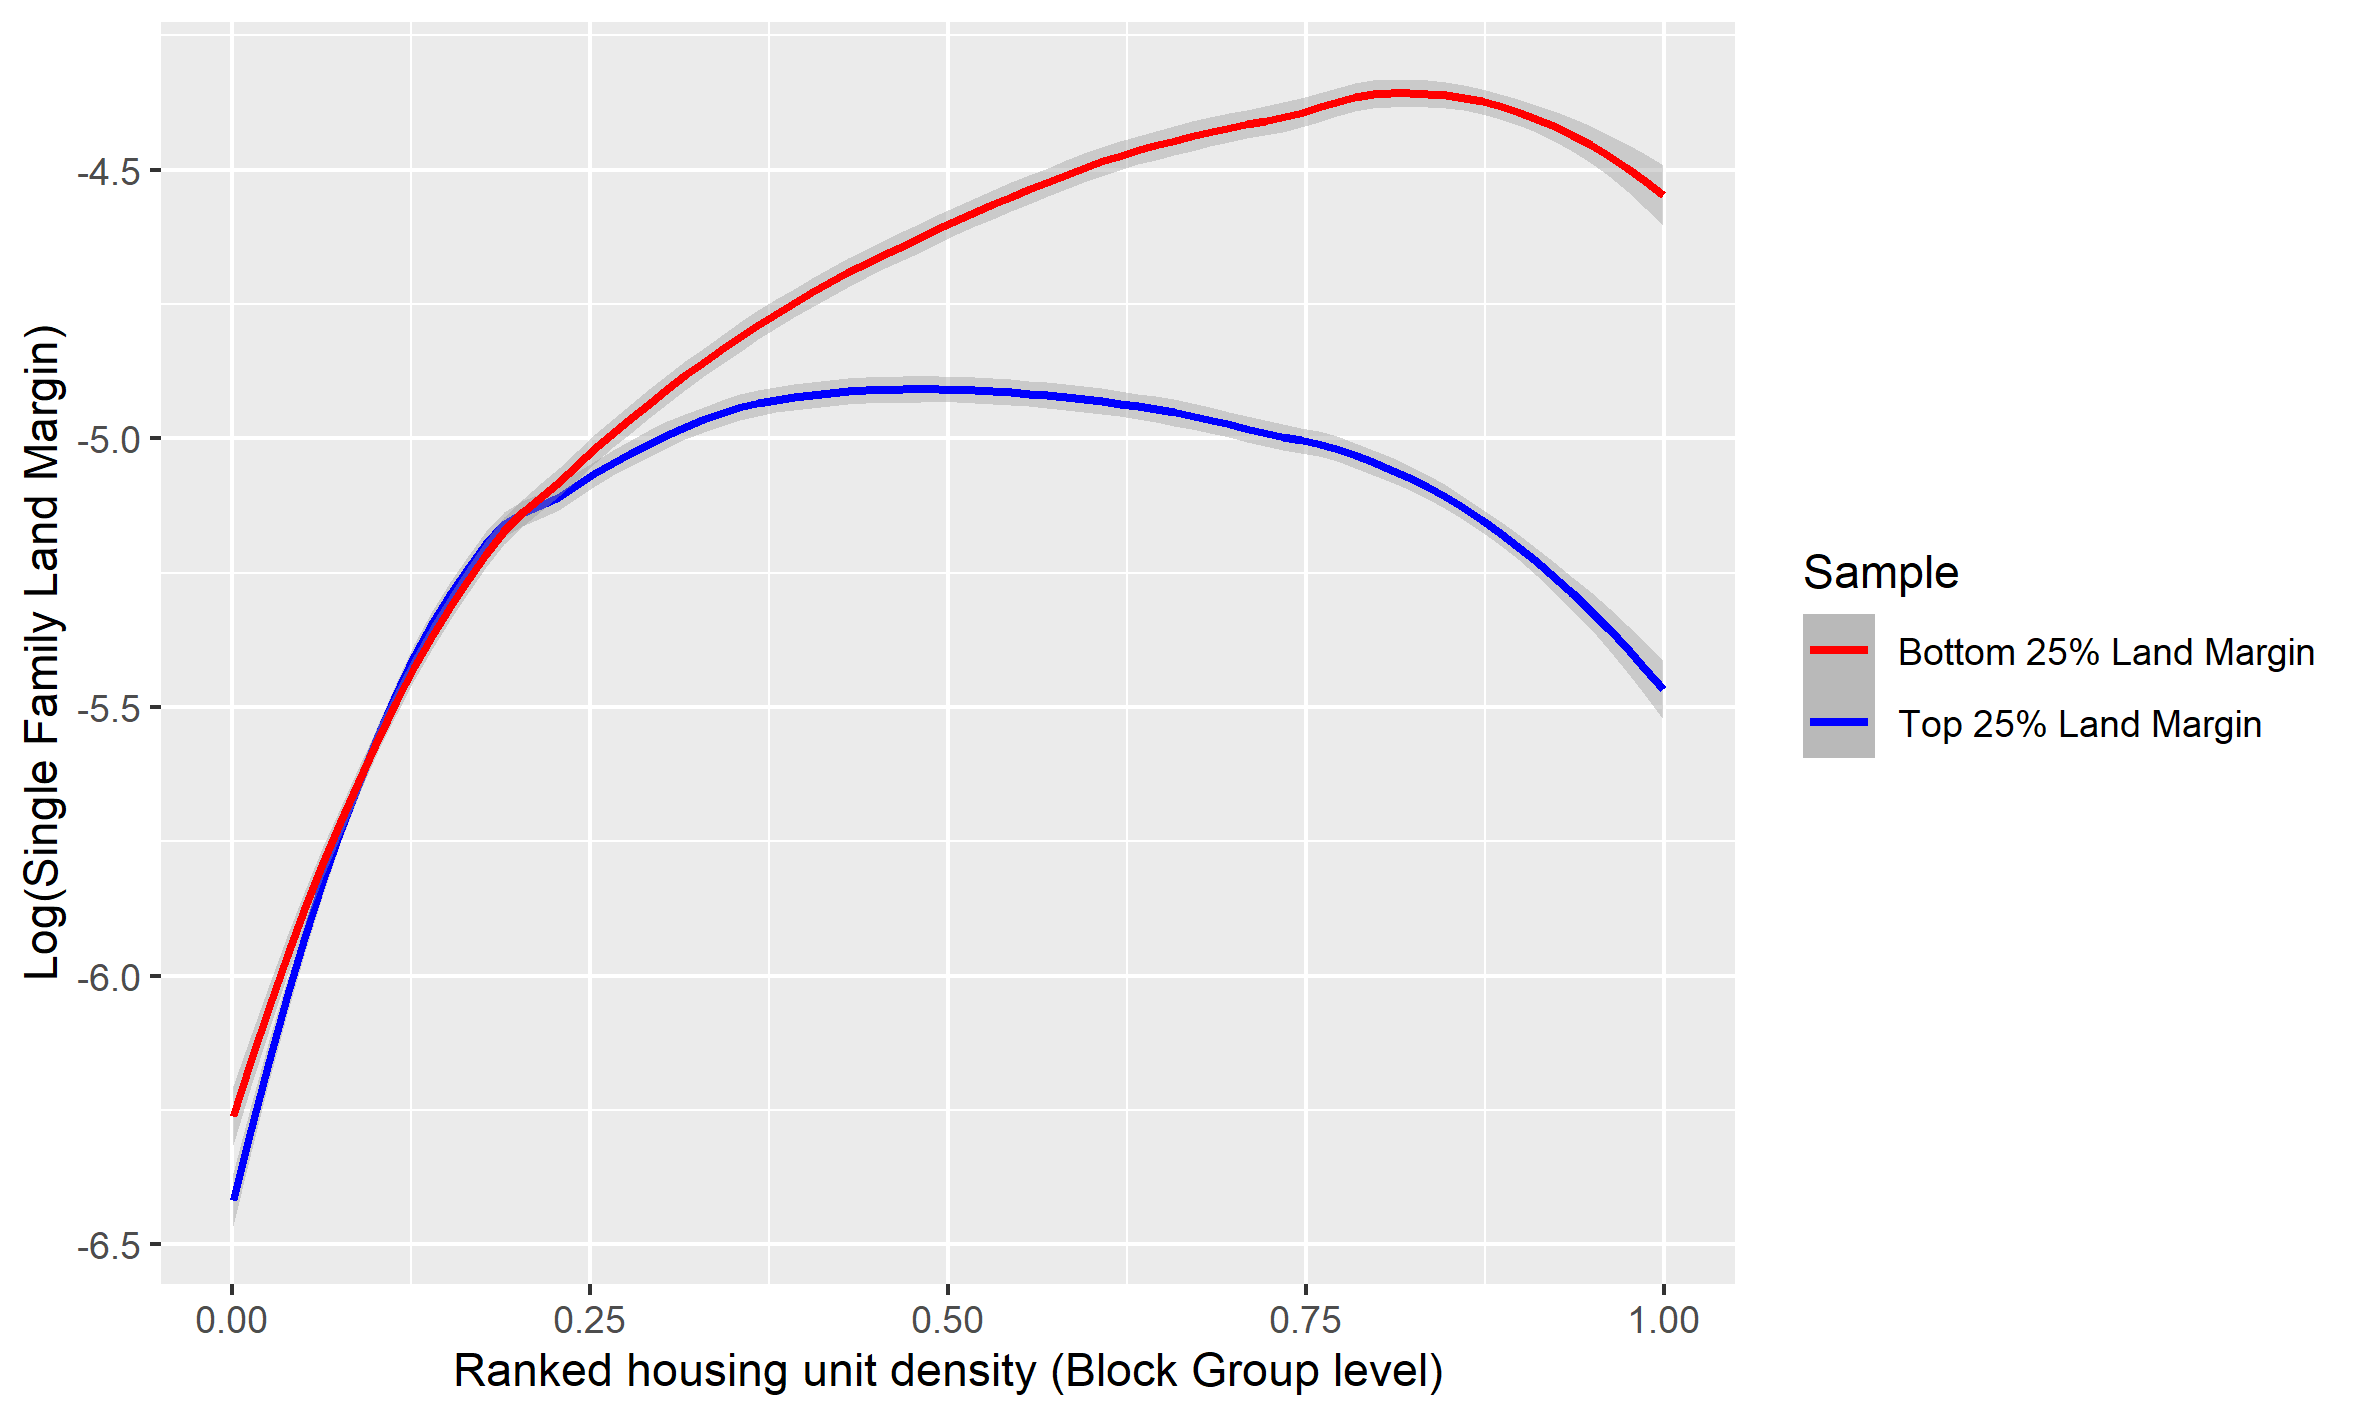
\includegraphics[width=0.7\textwidth, height=0.5\textheight]{SingleFamilyLand.png}}
\end{frame}

\begin{frame}{Takeaways:}
\begin{itemize}
	\color{black}
	\item Takeaways:
	\begin{enumerate}
		\item Both land and density margins contribute to low single family density, but a majority of the effect comes from the land margin. 
		\item Suggests that single family homes crowd out land that could be used for other types of structures, but that this effect is modest. 
	\end{enumerate}
\end{itemize}
\end{frame}

\begin{frame}{Fact 4: Stronger income sorting on housing unit density}
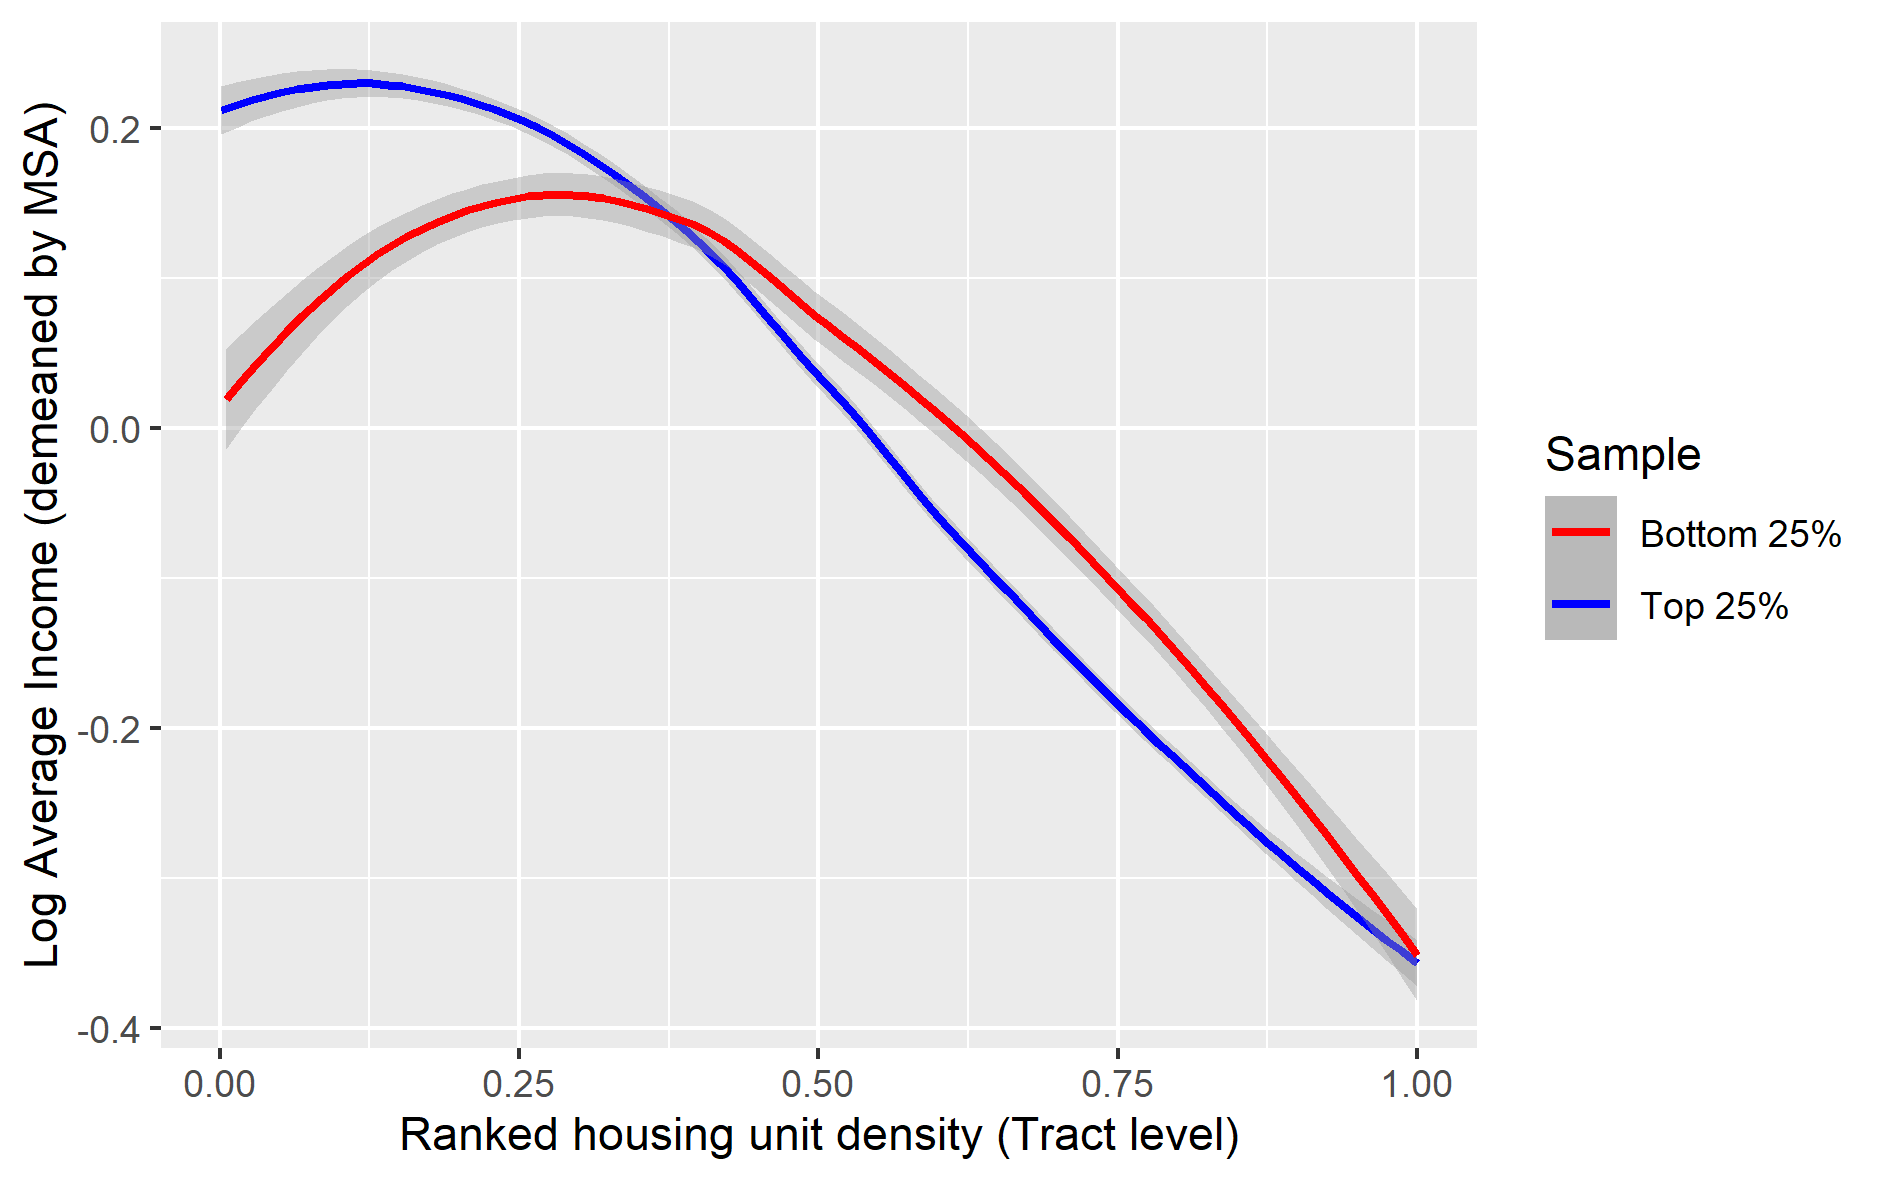
\includegraphics[width= \textwidth]{income.png}
\end{frame}

\begin{frame}{The Model In Words}
\begin{itemize}
	\color{black}
	\itemsep1em
	\item Population differences (which cause higher housing prices) reallocate households away from neighborhoods with minimum lot sizes and toward neighbourhoods with lax zoning policy. \pause
	\item \color{red}Interpretation\color{black}: causes disproportionate increases in high density structures (like condominiums) and preserves low density structures (like single family homes). \pause
	\item This process causes additional welfare inequality for low income households, and harms relative to Pareto efficient outcome. \pause
	\item \color{red} Abstracts from Tiebout motives for zoning as in \cite{calabresetal}, as well as congestion/agglomeration externalities present in \cite{berlinwall}. 
\end{itemize}
\end{frame}

\begin{frame}{Model}
	\begin{itemize}
		\color{black}
		\itemsep1em
		\item Closed city, two (exogenous) neighbourhoods $S$ and $N$, indexed by $i$. Multiplicative commuting costs $i$ given by $(1-\tau_{i})$. \pause
		\item Mass $L$ of households with labour productivity $z \in (0, \infty)$. Distributed with CDF $F$. Wages $w$ are exogenous. \pause
		\item $S$ has a minimum lot size, permitting a maximum of $\bar{U}$ households \pause
		\item Absentee landowners who don't consume housing. \pause
		\item Households consume local housing with Cobb-Douglas share $\beta$  \pause
		\item Developers possess Cobb-Douglas technology with land share $\alpha$. Capital supplied with perfect elasticity at exogenous cost $r$. 
	\end{itemize}
\end{frame}

\begin{frame}{Zoning and the Developer's Problem}
	\begin{itemize}
		\color{black}
		\item Let $P_{i}$ be the price of an efficiency unit of housing in neighbourhood $i$. 
		\item Issue: Housing developers in $S$ have to respect the minimum lot size. 
		\item Assumption: They can \textit{guarantee} to profit maximize ex-post if they enforce a \textit{minimum quality} $A^{\star}$ satisfying 
		\begin{equation}
			A^{\star} = P_{S}^{\frac{1-\alpha}{\alpha}}(\bar{U})^{-1}
		\end{equation}
		\item Assumption: households internalize $A^{\star}$ when choosing a neighbourhood and how much housing to consume.
	\end{itemize}
\end{frame}

\begin{frame}{How lot sizes work in this model}
\includegraphics[width= \textwidth]{BidRent.png}
\end{frame}

\begin{frame}{How lot sizes work in this model}
\includegraphics[width=\textwidth]{BidRentMinLot.png}
\end{frame}

\begin{frame}{Conclusion}
\begin{itemize}
	\itemsep1em
	\item The distributions of housing unit density in superstar cities are fundamentally different from others. 
	\item These differences appear to be driven by the presence of single family homes, with inadequate supply responses of medium density homes in the middle of the distribution.
	\item Single family homes crowding out land plays modest part in explaining this phenomenon. 
	\item I argue minimum lot sizes outside of central cities are important drivers of these facts. 
\end{itemize}
\end{frame}


\appendix
\begin{frame}{Appendix: Two Key Lemmas}
	\itemsep1em
	\begin{lem}
		In any equilibrium,$\frac{P_{S}}{P_{N}} \leq \bigg[\frac{1-\tau_{S}}{1-\tau_{N}}\bigg]^{\frac{1}{\beta}}$ \pause
	\end{lem}
	\begin{lem}
		If, in equilibrium, $\frac{P_{S}}{P_{N}} < \bigg[\frac{1-\tau_{S}}{1-\tau_{N}}\bigg]^{\frac{1}{\beta}}$, then there exists some $\bar{z}$ such that every $z < \bar{z}$ chooses neighbourhood $N$ and every $z > \bar{z}$ chooses neighbourhood S. 
	\end{lem}
\end{frame}


\begin{frame}{Appendix: Superstars and the Missing Middle}
	\begin{prop}
		(Superstars and the Missing Middle) Consider two cities with masses $L'$ and $L$ of households and cut-offs $\bar{z}'$ and $\bar{z}$ that come from an equilibrium satisfying $\frac{P_{S}}{P_{N}} < \bigg[\frac{1-\tau_{S}}{1-\tau_{N}}\bigg]^{\frac{1}{\beta}}$. Then:
		\begin{enumerate}
			\item If $L' - L$ is sufficiently large, then $\bar{z}' > \bar{z}$.
			\item  If $L' - L$ is sufficiently large, then $\frac{L'_{N}}{L'_{S}} > \frac{L_{N}}{L_{S}}$ 
		\end{enumerate} 
		where $L_{i}$ is the equilibrium mass of households in $i$.
	\end{prop}	
\end{frame}


\begin{frame}{Appendix: Regressive Consequences of the Missing Middle}
	\begin{itemize}
		\item Let $V(z)$ be the welfare of a type $z$ household
		\item Define $\tilde{V}(z) := \frac{V(z)}{z}$. 
		\item Crucial: $\tilde{V}(z)$ is \textit{constant in an equilibrium with no minimum lot sizes}. 
		\item Minimum lot sizes cause additional consumption inequality: 
	\end{itemize}
\begin{prop}\label{regressive}
	(Regressive consequences of the Missing Middle) Consider a city with a cutoff $\bar{z}$ that comes from an equilibrium satisfying $\frac{P_{S}}{P_{N}} < \bigg[\frac{1-\tau_{S}}{1-\tau_{N}}\bigg]^{\frac{1}{\beta}}$. Then, $\tilde{V}(z) < \tilde{V}(z')$ for all $z$, $z'$ satisfying $z < \bar{z} < z'$.
\end{prop}
\end{frame}

\begin{frame}{Appendix: Regressive Consequences of the Missing Middle II}
\begin{itemize}
	\item Previous proposition says nothing about how low income households are made worse off relative to a Pareto optimal equilibrium with no lot sizes. So... \pause
\end{itemize}
\begin{prop}\label{regressiveII}
	(Regressive consequences of the Missing Middle II) Consider a city with a cutoff $\bar{z}$ that comes from an equilibrium satisfying  $\frac{P_{S}}{P_{N}} < \bigg[\frac{1-\tau_{S}}{1-\tau_{N}}\bigg]^{\frac{1}{\beta}}$. If $\bar{z}$ is sufficiently large, then for all $z < \bar{z}$, households of type $z$ are made worse off relative to an equilibrium with no minimum lot sizes. 
\end{prop}
\end{frame}

\bibliography{references.bib}
\end{document}